%====================================================================
%====================================================================
\subsection*{Bipartite expected degree distribution}
\frame{\frametitle{Bipartite expected degree distribution} \label{sec:BEDD}

  \begin{tabular}{rccc}
    & & $h_0(v) =$ & $h(v) =$ \\
    \multicolumn{2}{c}{
      \begin{tabular}{p{0.3\textwidth}} 
        $$
        U_i, V_j \sim \Ucal[0, 1]
        $$
        $$
        Y_{ij} \sim \Bcal(\emphase{\rho} \; \emphase{g}(U_i) \; \emphase{h}(V_j))
        $$
        $$
        \textstyle{\int g = \int h = 1}
        $$
      \end{tabular}
%       $\begin{array}{rl}
%         \Pbb\{Y_{ij} = 1 \mid U_i, V_j\} & = \rho \; g(U_i) \; h(V_j) \\ \\
%         \Esp (Y_{i+} \mid U_i) & = n \; \rho \; g(U_i) \\ \\
%         \Esp (Y_{+j} \mid V_j) & = m \; \rho \; g(V_i) 
%       \end{array}$
    } 
    &
    \begin{tabular}{c} 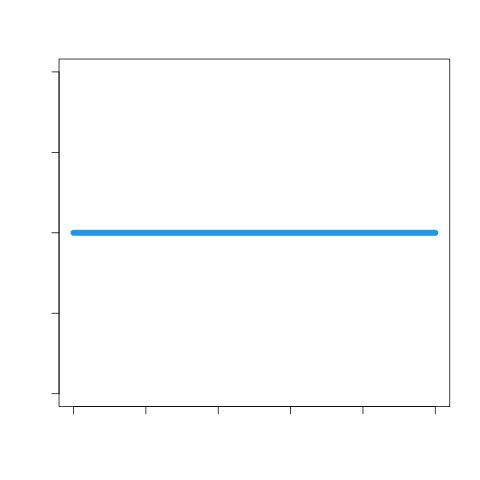
\includegraphics[width=.15\textwidth, trim=30 30 30 30, clip=]{\fignet/FigMotifsBEDD-dist-h10} \end{tabular} &
    \begin{tabular}{c} 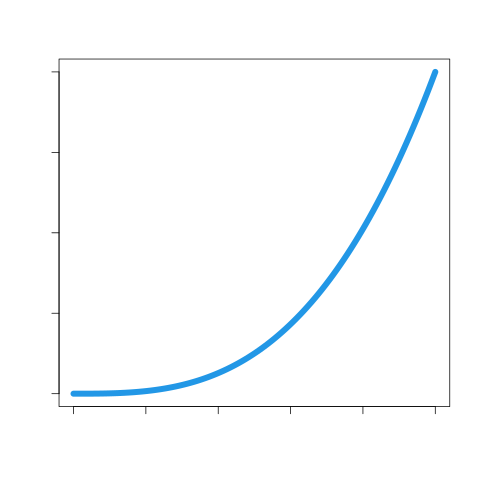
\includegraphics[width=.15\textwidth, trim=30 30 30 30, clip=]{\fignet/FigMotifsBEDD-dist-h40} \end{tabular} \\
    \begin{tabular}{r} $g_0(u) =$ \end{tabular} &
    \begin{tabular}{c} 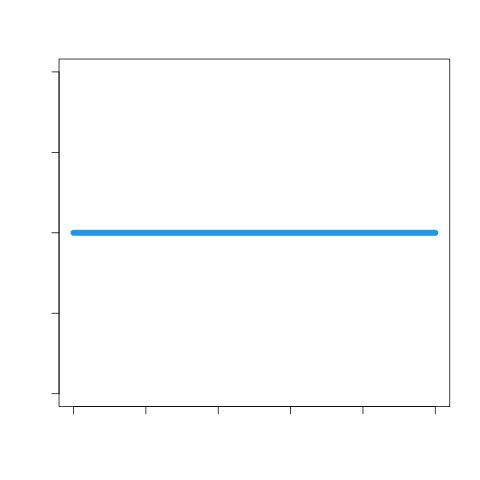
\includegraphics[width=.15\textwidth, trim=30 30 30 30, clip=]{\fignet/FigMotifsBEDD-dist-g10} \end{tabular} &
    \begin{tabular}{c} 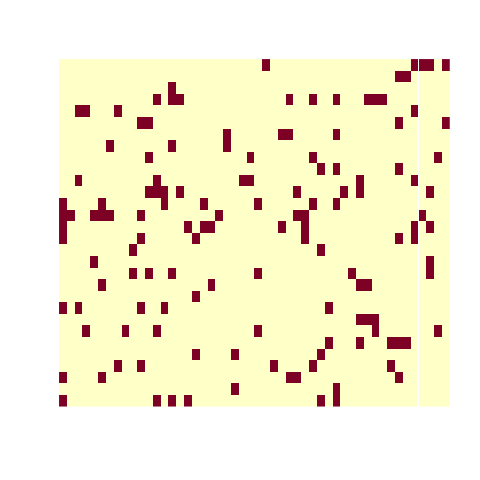
\includegraphics[width=.15\textwidth, trim=30 30 30 30, clip=]{\fignet/FigMotifsBEDD-adj-g10-h10} \end{tabular} &
    \begin{tabular}{c} 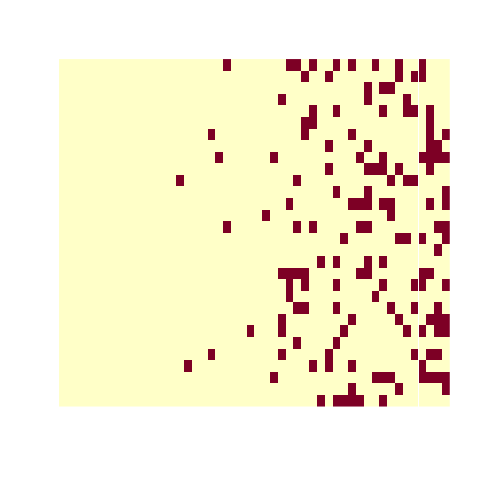
\includegraphics[width=.15\textwidth, trim=30 30 30 30, clip=]{\fignet/FigMotifsBEDD-adj-g10-h40} \end{tabular} \\
    \begin{tabular}{r} $g(u) =$ \end{tabular} &
    \begin{tabular}{c} 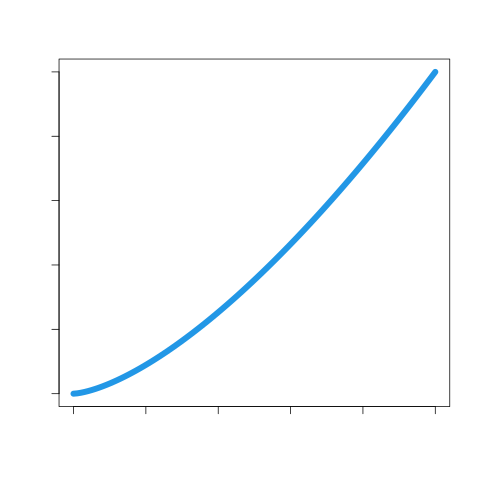
\includegraphics[width=.15\textwidth, trim=30 30 30 30, clip=]{\fignet/FigMotifsBEDD-dist-g25} \end{tabular} &
    \begin{tabular}{c} 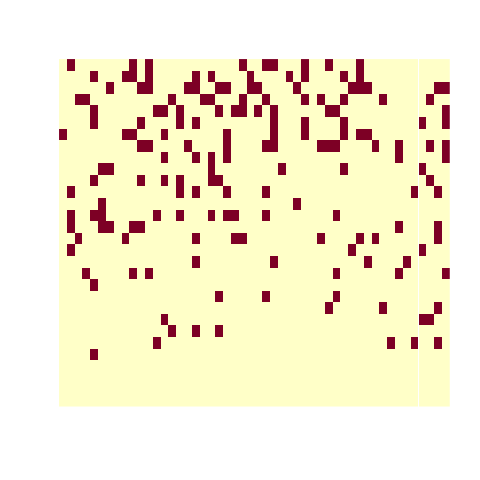
\includegraphics[width=.15\textwidth, trim=30 30 30 30, clip=]{\fignet/FigMotifsBEDD-adj-g25-h10} \end{tabular} &
    \begin{tabular}{c} 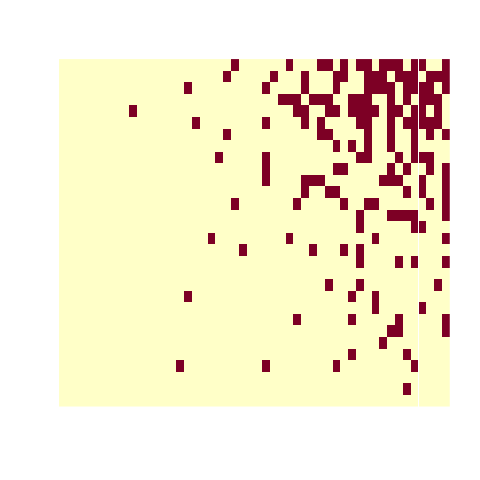
\includegraphics[width=.15\textwidth, trim=30 30 30 30, clip=]{\fignet/FigMotifsBEDD-adj-g25-h40} \end{tabular} \\
  \end{tabular}
  
  \pause
  \begin{itemize}
    \item No preferred or avoided specific connexion
    \item \emphase{Graph-exchangeable} model: pollinators (and plants) can be permuted 
    \item Bipartite version of the expected degree distribution \refer{ChL02}
    \item Expected degrees: $\Esp(Y_{i+} \mid U_i) = n \rho g(U_i)$, $\Esp(Y_{+j} \mid V_j) = m \rho h(V_j)$. \goto{sec:nullModel}
  \end{itemize} 
  
}
%====================================================================

%====================================================================
%====================================================================
\subsection{Motif count distribution}
%==================================================================
\frame{\frametitle{Motif count}

  \paragraph{Couting motifs\footnote{Not in the way of the \url{bmotif} package \refer{SSS19}}.} For a given motif $s$ with $p_s$ top nodes and $q_s$ bottom nodes:
  \begin{itemize}
    \item Choose $p_s$ nodes among $m$ and $q_s$ nodes among $n$;
    \item \pause Try the \emphase{$r_s$} {\sl automorphisms} = non-redundant permutations
    $$
    \includegraphics[width=.07\textwidth]{\fignet/FigMotifsBEDD-motif9-automorphism1}
    \includegraphics[width=.07\textwidth]{\fignet/FigMotifsBEDD-motif9-automorphism2}
    \includegraphics[width=.07\textwidth]{\fignet/FigMotifsBEDD-motif9-automorphism3} 
    \includegraphics[width=.07\textwidth]{\fignet/FigMotifsBEDD-motif9-automorphism4}
    \includegraphics[width=.07\textwidth]{\fignet/FigMotifsBEDD-motif9-automorphism5}
    \includegraphics[width=.07\textwidth]{\fignet/FigMotifsBEDD-motif9-automorphism6} 
    $$
    \item The number of possible 'positions' is then 
    $$
    c_s := 
    \left(\begin{array}{c}m \\ p_s\end{array}\right)
    \times \left(\begin{array}{c}n \\ q_s\end{array}\right)
    \times r_s;
    $$ 
    \item \pause Try all positions $\alpha = 1, \dots c_s$, and count the number of matches:
    $$
    N_s = \sum_{\alpha = 1}^{c_s}\Ibb\{\text{motif $s$ matches at position $\alpha$}\}.
    $$
  \end{itemize}

  \bigskip \pause
  \paragraph{Expected count.} $\Esp(N_s) = c_s \phi_s$, with
  $$
  \phi_s = \text{matching probability} = \text{'motif probability'}
  $$
  
}

%==================================================================
\frame{\frametitle{Motif probability} 

  \bigskip 
  \paragraph{Motif probability $\overline{\phi}_s$ under BEDD\footnote{Consider here induced motifs  (only the presence of the prescribed edges is required) $\neq$ exact motif}.} Need to integrate wrt $Z = (U, V)$.
  
  \bigskip \pause
  \paragraph{An example.} Consider the motif $s = \includegraphics[width=.06\textwidth, trim=100 200 100 0]{\fignet/FigMotifsBEDD-motif9}$ with $p_s = 2$ and $q_s = 3$, we have
  \begin{align*}
    \overline{\phi}_s
    & = \int\int\int\int\int \rho^4 g(u_1) g(u_2)^3 h(v_1) h(v_2) h(v_3)^2 \d u_1 \d u_2 \d v_1 \d v_2 \d v_3 \\
    & = \left. \left(\int \rho^3 g(u_2)^3 \d u_2\right) \left(\int \rho^2 h(v_3)^2 \d v_3\right) \right/ \rho \qquad \qquad \goto{back:motifProba}  \\
    & = \left. \left(\text{bottom 3-star probability}\right) \times \left(\text{top 2-star probability}\right) \; \right/ \left(\text{edge probability}\right)
  \end{align*} \label{sec:motifProba}

  \bigskip \pause
  \paragraph{A favourable configuration.}
  \begin{itemize}
    \setlength{\itemsep}{.75\baselineskip}
    \item Edge and star probabilities contain all information.
    \item Unbiased estimates are given by their respective empirical frequencies $F = N / c$ \\
    (sufficient statistics of the BEDD model).
    \item The integration wrt $Z = (U, V)$ is implicitly achieved (without estimating $g$ and $h$).
  \end{itemize}

}

%==================================================================
\frame{\frametitle{Some more results}

  \bigskip
  \paragraph{Moments of the count.}
  \begin{itemize}
  \setlength{\itemsep}{.75\baselineskip}
  \item \emphase{Mean:} $\Esp(N_s) = c_s \times \overline{\phi}_s$ 
  \item \emphase{Variance:} Same game, requires to evaluate ${\Esp(N_s ^2) = \Esp\left(\sum_\alpha \text{match}_{s\alpha} \right)^2}$ \\
  \ra Need to consider overlaps between positions ({\sl super-motifs}: \refer{PDK08} \goto{back:superMotifs})  \label{sec:motifMoments}
  $$
  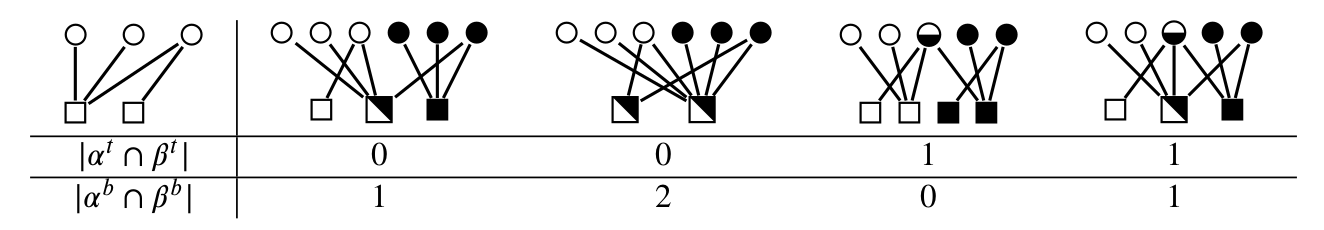
\includegraphics[width=.8\textwidth, trim=0 25 0 5, clip=]{\fignet/OLR22-EJS-Fig2}
  $$ 
  \ra Compute the respective expected count in the way as for other motifs 
  \item \emphase{Covariance:} Same game to compute $\Cov(N_s, N_{s'})$
  \end{itemize}
  
  \bigskip \bigskip \pause
  \emphase{Proposition: Asymptotic normality \refer{OLR22}.} Under {\BEDD}, for non-star motifs, 
  \begin{itemize}
%   \setlength{\itemsep}{.75\baselineskip}
  \item Under sparsity conditions ($\rho \; \propto \; m^{-a} n^{-b}$): 
  $$
  (N_s - \widehat{\Esp}(N_s)) \left/ \sqrt{\widehat{\Var}(N_s)} \right. \quad \overset{m, n \rightarrow \infty}{\longrightarrow} \quad \Ncal(0, 1)
  $$
  \item Account for plug-in for moderate network size ($\Delta$-method):
  $$
  \left(N_s - \widehat{\Esp}(N_s) + \widehat{\Bias}\left(\widehat{\Esp}(N_s)\right)\right) \left/ \sqrt{\widehat{\Var}(N_s - \widehat{\Esp}(N_s))} \right. \quad \overset{m, n \rightarrow \infty}{\longrightarrow} \quad \Ncal(0, 1)
  $$ 
  \end{itemize}

}

%====================================================================
%====================================================================
\subsection{Networks comparison in space and time}
\frame{\frametitle{Networks comparison in space and time} }
%====================================================================

%====================================================================
\frame{\frametitle{Experimental design} 

  Joint work with Natasha de Manincor et Fran\c{c}ois Massol

  \bigskip
  \paragraph{Question.} 
  Does the structure of plant-pollinator network vary in space and time?
  
  \bigskip \pause
  \paragraph{Design.} 
  \begin{itemize}
    \setlength{\itemsep}{.75\baselineskip}
    \item 3 French regions (Hauts-de-France, Normandie and Occitanie), 2 sites / region
    \item 2 years, 7 months / year
    \item $3 \times 2 \times 2 \times 7 \simeq 82$ networks 
  \end{itemize}

  \bigskip \pause
  \paragraph{Approach.} Distance-based embedding:
  \begin{itemize}
    \setlength{\itemsep}{.75\baselineskip}
    \item Define a network distance (gathering all motifs)
    \item Use (permutation-based) multivariate analysis of variance to test spatial or temporal effects ('Adonis', \refer{McA01,ZaS06})
  \end{itemize}

}
%==================================================================
\frame{\frametitle{Comparing network imbalances}

  \bigskip
  \paragraph{Question.} Do network $A$ and $B$ share the same imbalance for pollinators?
  
  \bigskip \pause
  \paragraph{Test statistic.} 
  \begin{itemize}
    \item Assume $A \sim BEDD(\rho^A, g^A, h^A)$ and $B \sim BEDD(\rho^B, g^B, h^B)$
    $$
    H_0 = \{g^A = g^B\}
    $$
    \item For motif $s$, with 
    $$
    \widehat{\Esp}_0(N_s^A) = \widehat{\Esp}_{\widehat{\rho}^A, \emphase{\widehat{g}^B}, \widehat{h}^A}(N^A_s), \qquad 
    \widehat{\Esp}_0(N_s^B)) = \widehat{\Esp}_{\widehat{\rho}^B, \emphase{\widehat{g}^A}, \widehat{h}^B}(N^B_s)
    $$
    we have
    $$
    W^{(g)}_s(A, B) = \frac{(N_s^A - \widehat{\Esp}_0(N_s^A)) - (N_s^B - \widehat{\Esp}_0(N_s^B))}{\sqrt{\widehat{\Var}_0(N^A_s) + \widehat{\Var}_0(N^B_s)}}
    \overset{H_0}{\sim} \Ncal(0, 1)
    $$ 
  \end{itemize}

  \bigskip \pause
  \paragraph{Network 'distance'} for pollinator imbalance
  $$
  D^{(g)}(A, B) = \sqrt{\sum_s W^{(g)}_s(A, B)^2}
  $$

}

%==================================================================
\frame{\frametitle{Results} \label{sec:adonisResults}
%   \newcommand{\fignatA}{/home/robin/RECHERCHE/RESEAUX/GOF-Network/Motif_Analysis_Natasha/Figures}
%   \newcommand{\fignatB}{/home/robin/RECHERCHE/RESEAUX/GOF-Network/Motif_Analysis_Natasha/Article/Figures}
  \newcommand{\tabnat}{/home/robin/RECHERCHE/RESEAUX/EXPOSES/2504-Montpellier/Tables}
  
  \paragraph{Pollinator imbalance $D^{(g)}$.} Anova table
  $$\small{
  \begin{tabular}{l|rrrrr}
    & Df & Sum Of Sqs & $R^2$ & F & Pr(\>F) \\ 
\hline
\emphase{InsectNb} & 1 & 69.9 & 0.2595 & 42.69 & \emphase{1e-05} \\ 
\emphase{PlantNb} & 1 & 31.17 & 0.1157 & 19.04 & \emphase{1e-05} \\ 
Year & 1 & 2.66 & 0.0099 & 1.62 & 0.22212 \\ 
\emphase{Month} & 6 & 24.8 & 0.092 & 2.52 & \emphase{0.00959} \\ 
\emphase{Region} & 2 & 8.67 & 0.0322 & 2.65 & \emphase{0.04531} \\ 
Year:Month & 6 & 4.81 & 0.0179 & 0.49 & 0.88756 \\ 
Year:Region & 2 & 5.51 & 0.0204 & 1.68 & 0.1787 \\ 
{\bf Month:Region} & 12 & 32.41 & 0.1203 & 1.65 & {\bf 0.06346} \\ 
Year:Month:Region & 12 & 27.26 & 0.1012 & 1.39 & 0.15884 \\ 
Residual & 38 & 62.22 & 0.2309 & &  \\ 
Total & 81 & 269.42 & 1 & & 

  \end{tabular}
  }$$

  \bigskip
  \begin{itemize}
    \setlength{\itemsep}{.75\baselineskip}
    \item \pause Because of small network sizes, need to correct for the number of insects and plants 
    \item \pause Significant effect of the region and the month, indicating changes of the insect imbalance both in space and time
    \item \pause The pattern is conserved from year to the next (not year effect)
    \item \pause No significant effect found for the plant imbalance distance $D^{(h)}$ 
  \end{itemize}

}

